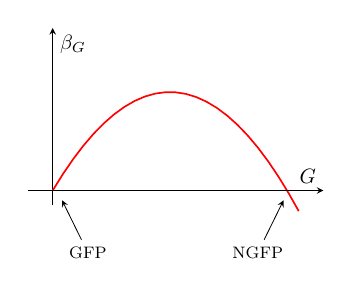
\begin{tikzpicture}[
    >=stealth,
    scale=0.75,
    thick
  ]

  \begin{axis}[
    width=5.0cm,
    height=3.0cm,
    scale only axis,
    major tick length=2pt,
    xlabel={$G$},
    ylabel={$\beta_G$},
    xmin= 0.0, xmax=2.1,
    ymin= 0.0, ymax=1.5,
    axis lines = middle,
    enlargelimits = true,
    ticks=none,
    legend cell align=left,
    legend pos=outer north east,
    clip=false
    ]

    \addplot[red,   domain=0:2.1, thick, ]{ 2*x - x^2 };
    \addplot[black, domain=-0.1:2.1, line width=0mm,  ]{ 0 };

    \node (gfp) at (axis cs:0.30,-0.5) [anchor=north] {\footnotesize GFP};
    \draw[->] (gfp) -- (axis cs:0.08,-0.1);

    \node (ngfp) at (axis cs:1.75,-0.5) [anchor=north] {\footnotesize NGFP};
    \draw[->] (ngfp) -- (axis cs:1.97,-0.1);

  \end{axis}


\end{tikzpicture}
